%TODO: CORREGIR COMANDOS PARA QUE SE VEAN CON VERB
%TODO: INTENTAR QUITAR LA MORRAYA QUE NO SIRVA
%TODO: INTENTAR NO REPETIR TANTAS COSAS EN EL EJERCICIO 3
%TODO: REVISAR DOCUMENTO PARA FALLOS ORTOGRAFICOS/GRAMATICALES
\documentclass{article}
\usepackage[utf8]{inputenc}
\usepackage[spanish]{babel}
\usepackage{graphicx, graphics, float, hyperref}
\usepackage{listings, subcaption}
\usepackage[a4paper, total={6in, 10in}]{geometry}

\title{SSO Práctica 4 Sesión 1}
\author{Andrés Merlo Trujillo}
\date{}
\hypersetup{
    colorlinks=true,
    linkcolor=black,
}

\begin{document}

\maketitle

\tableofcontents

\newpage
%\addcontentsline{toc}{section}{Ejercicio 1}
%\section*{Ejercicio 1}
%\begin{figure}[H]
%    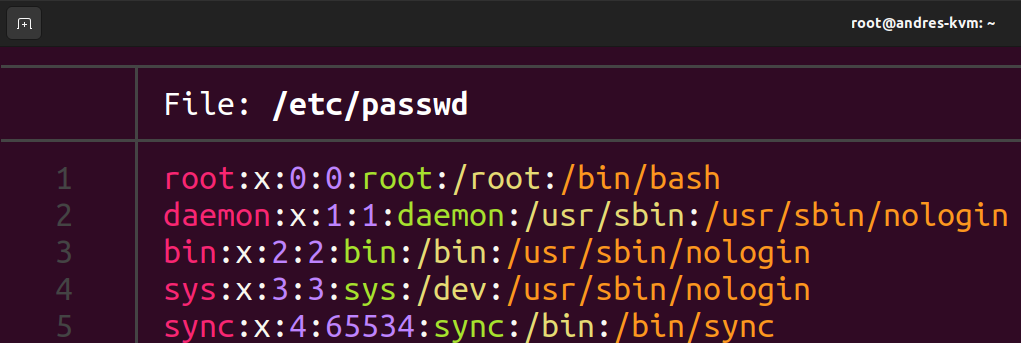
\includegraphics[width=\textwidth]{imagenes/passwdfile.png}
%    \caption{Ejemplo de entradas en el archivo.}
%\end{figure}

\addcontentsline{toc}{section}{Ejercicio 1}
\section*{Ejercicio 1}

Voy a crear una partición con el sistema de archivos FAT32 (debido a problemas con Autopsy que me surgieron en los siguientes ejercicios)

Y ahora a modo de realismo, voy a copiar las imagenes usadas durante estas practicas y un archivo dentro de la carpeta ``mis trabajos'' denominado ``amenaza.txt'' con una frase que amenace.

%Foto de la carpeta con archivos y del archivo amenaza

A continuacion elimino esse archivo y desmonto el disco para suponer que he recibido el pendrive asi y para que no pueda realizarle mas modificaciones.

Ahora voy a seguir los pasos indicados en el guion de practicas, por tanto, lo primero que hay que hacer es obtener la estructura interna de particiones con la orden \verb|fdisk -l /dev/sdX > fdisk.disco1| siendo la X la letra asignada al disco, en mi caso es a. (se puede comprobar con la orden \verb|fdisk -l| o \verb|lsblk|).

%foto de la salida del comando

Lo siguiente que hay que hacer es crear una imagen forense del disco para evitar invalidar el contenido del pendrive y trabajar de forma segura sobre una copia. Esto se realiza mediante la orden \verb|dd if=/dev/sda1 of=imagen.disco1 bs=512|.

%salida de dd

Ahora es necesario poner la imagen del disco a solo lectura con la orden \verb|chmod 444 imagen.disco1|.

El siguiente paso, que es copiar la imagen a otro disco no es necesario, ya que se puede trabajar directamente sobre la imagen como explicare a continuacion. Ahora se debe montar la imagen con la orden \verb|mount imagen.disco1 /mnt -o noexec,loop|, y al hacer \verb|lsblk -f| se puede ver que está montado correctamente.

%foto de la salida de lsblk
%caption{Se puede ver que el nombre que tiene es \texttt{loop2} y que se ha montado correctamente en el punto de montaje indicado.}

Ahora es necesario verficar la integridad de los datos del pendrive antes y despues de completar el analisis, para ello se usa la orden \verb|sha1sum /dev/sda1 > SHA.disco1|.

%foto de sha1sum

Y ahora, voy a realizar lo mismo, pero sobre cada archivo. En este caso se debe hacer sobre la imagen porque al montar el pendrive puede darse el caso de que el hash cambie. Para ello, desde la raiz de la imagen montada, se debe hacer con la orden \verb|find . -type f -exec sha1sum {} \; > SHA.listaArchivos|.

%salida del comando con bat

Y se puede realizar la verficiacion con la orden \verb|sha1sum -c ~/SHA.listaArchivos| (se debe estar dentro de la raiz de la imagen)

%salida del comando.

Ahora se puede proceder con seguridad a encontrar el archivo eliminado anteriormente. Para ello, es necesario crear un fichero con las palabras claves mas probables que se encuentren. El fichero tiene la siguiente forma:

%slaida

Ahora con la orden \verb|grep -aibf palabrasClave imagen.disco1 > aciertos.txt| se puede realizar la busqeuda en la imagen:

%salida en aciertos.txt

Como se puede ver, aparece la frase ``Esto es una amenaza, si no nos da algo de dinero publicamos el contenido de su pendr...'', indicando que ha habido una amenaza.

Por ultimo, para asegurarse, se puede usar el comando \texttt{xxd -s 299892684 imagen.disco1 | less} para verlo en la propia imagen:

%salida del comando

Y efectivamente, aqui tamvien aparece.

\addcontentsline{toc}{section}{Ejercicio 2}
\section*{Ejercicio 2}

EN esta parte es necesario utilizar la herramienta ``GuyMager'' para obtener una imagen forense del mismo pendrive. POr tanto, se descarga el programa mediante \verb|apt| y se abre.

%foto de inicio.

Y se pulsa con click derecho en el dispositivo que se quiera realizar la imagen, en mi caso \verb|/dev/sda|, y le damos a ``Acquire image''.

%ventana nueva

Y ahora simplemente rellenamos los campos que se piden y al final quedan asi:

%foto de esto relleno

Por ultimo, es necesario darle a ``Start'' para que comience el proceso.

%foto del progreso
%caption{Progreso de creacion de imagen forense.}

Al finalizar, se puede ver que ha generado varios trozos de la imagen del pendrive.

%foto

\addcontentsline{toc}{section}{Ejercicio 3}
\section*{Ejercicio 3}

\textbf{NOTA: }La version de Autopsy para Linux con la interfaz web no era capaz de detectar las particiones de la imagen creada con la herramienta del ejercicio anterior, por lo que he decidido usar la ultima version de Autopsy que sí la detecta.

\addcontentsline{toc}{subsection}{Apartado A}
\subsection*{Apartado A}

Cuando se ejecuta Autopsy aparece la siguiente pantalla:

%foto pantalla

Ahora le damos a ``New Case'' y se le elige un nombre, la ubicacion, el numero de caso, algunso datos del examinador:

%fotos rellenas

Al darle a Finish, aparece otra venta en la que se pide añadir una fuente de datos, en este caso al imagen creada, para ello se elige ``Disk Image or VM File'' y se elige el primer fragemnto de la imagen:

%fotos rellenas

Tras que el programa procese la imagen, aparece el siguiente panel:

%foto panel

Y ahora es necesario darle a Data Sources $\rightarrow$ imagenPendrive.E01\_1 Host $\rightarrow$ imagenPendrive.E01 $\rightarrow$ vol4.

%foto salida

Como se puede ver, hay 3 particiones que hacian que versiones antiguas de Autopsy (con interfaz web) no pudiesen detectar el sistema de archivos correctamente y solo funcionasen en modo raw.

Ahora bien, hay dos opciones de ver archivos eliminados, la primera es yendo a la ubicacion donde estaba el archivo, y la segunda es dandole al boton del panel de la izquierda ``Deleted Files''.

%foto de deleted files y el otro

Y como se puede ver detecta el archivo eliminado del pendrive y muestra su informacion.

%SECCION DE IMAGENES DE WINDOWS

\addcontentsline{toc}{subsection}{Apartado B}
\subsection*{Apartado B}

\textbf{NOTA: }Ahora voy a usar la versión de Windows de Autopsy, ya que me he dado cuenta que contiene muchas mas opciones que la version de Linux no tiene (como ponerle nombre a las cuentas del sistema operativo, que en Linux no pasa).

\addcontentsline{toc}{subsubsection}{¿Cuándo se creó la hoja de cálculo?}
\subsubsection*{¿Cuando se creó la hojra de calculo?}

Lo primero de todo es encontrar la hoja de calculo en la imagen del ordenador de Jean. Es posible buscarla dandole a File Views $\rightarrow$ By Extension $\rightarrow$ Documents $\rightarrow$ Office.

%foto
%caption{Como se puede observar, es el documento que ha sido filtrado}

AHora hay qeu darle a la pestaña ``File Metadata'' donde se indican todos los datos relacionados con el documento.

%foto

Se puede ver que la hoja de calculo fue creada el \textbf{20 de julio de 2008 a las 03:28:03 CEST}.

Ademas, en la pestaña ``Text'', justo debajo del contenido del documento, aparecen mas datos interesantes.

%foto

El mas notable es que fue creado por Alison Smith y que hay otra fecha de creacion distinta a la pestanña de los metadatos, pero personalmente creo que es mejor fiarse de la de metadatos, ya que estos datos pueden ser modificados.

\addcontentsline{toc}{subsubsection}{¿Como llegó de su computador al sitio web de la competencia?}
\subsubsection*{¿Como llegó de su computador al sitio web de la competencia?}

Sabiendo los testimonios de los posibles implicados, se puede intuir que Jean envió por error la hoja de cálculo a otra persona, posiblemente a alguien de la empresa de la competencia.

Para tener pruebas fehacientes de esto, podemos mirar el historial de correos de Jean, para ello, nos vamos a Data Artifacts $\rightarrow$ E-Mail Messages $\rightarrow$ Default $\rightarrow$ Default.

%foto overview

Tras mirar la conversacion entre Jean y Alice, pidiendole a Jean que trabaje y que no mande correos extraños que parecen SPAM, aparece un correo muy interesante de Alison.

%fotos hacker
%caption para una de ellas: Se puede ver que le insiste a Jean que le envie la informacion y le dice que no se lo diga a nadie.

Además, se ve que Jean le manda la hoja de calculo que se ha filtrado y al dia siguiente algunos empleados le preguntan que por que su informacion esta en internet, preguntandole a Jean que si la que hay sobre el es correcta. Por tanto se puede asumir que el correo de Alison ha sido comprometido y ha sido usado de manera maliciosa para obtener estos datos.

La conclusion final a esta pregunta es que Jean mandó al correo de Alison la hoja de calculo, pero al estar mal configurado (de manera malintencionada o no) fue enviado al atacante.


\addcontentsline{toc}{subsubsection}{¿Quién más de la compañía está involucrado?}
\subsubsection*{¿Quién más de la compañía está involucrado?}

Es difícil de saber, pero se sabe claramente que el correo de Alison tuvo un problema de configuración y estaba usando otra direccion de correo (alex@m57.biz) en el momento del ataque. Esto puede indicar que algún empleado obtuvo acceso al ordendador de Alison y ``desconfiguró'' su correo, dejando vía libre para poder usar el real. Puede que haya sido otro empleado descontento con la empresa que haya usado el correo de Alison para obtener la informacion, pero no se sabe a ciencia cierta.

\end{document}
